% THIS TEMPLATE IS A WORK IN PROGRESS

\documentclass[polish, a4paper]{article}
\usepackage[a4paper,left=3cm,right=3cm,top=3cm,bottom=1.5cm]{geometry}
\usepackage[T1]{fontenc}
\usepackage[polish]{babel}
\usepackage[utf8]{inputenc}
\usepackage{hyperref}
\usepackage{fancyhdr}
\usepackage{float}
\usepackage{graphicx}
\usepackage{titling}
\usepackage{wasysym}
\usepackage{caption}
\usepackage{pgfplots}
\usepackage{pgfplotstable}
\usepackage{filecontents}
\usepackage{csvsimple}
\usepackage{textcomp}
\usepackage{gensymb}
\usepackage{etoolbox}
%\usepackage{siunitx}
\graphicspath{ {./} }
\pagestyle{fancy}

\setlength{\droptitle}{-1in}

%\lhead{\includegraphics[width=0.2\textwidth]{nyush-logo.pdf}}

  \lhead{Maciej Kaszkowiak}
  \chead{Adresacja IP}
  \rhead{
  151856}


%%%% PROJECT TITLE
\title{Adresacja IP \\
        \Large \emph{Sprawozdanie nr 1 z przedmiotu Sieci Komputerowe}}

%%%% NAMES OF ALL THE STUDENTS INVOLVED (first-name last-name)
\author{Maciej Kaszkowiak, 151856, zadania wykonane 4 marca 2023}

\date{\vspace{-5ex}} %NO DATE


\begin{document}


\maketitle
%\thispagestyle{titlepage}

\tableofcontents

\section{Zadanie 1}

Dany jest adres 100.0.100.50/28.

\begin{enumerate}
\item{Oblicz adres sieci dla powyższego adresu.}
\item{Wskaż adres rozgłoszeniowy sieci.}
\item{Ile komputerów można zaadresować w tej sieci?}
\end{enumerate}

\subsection{Obliczenia}

50 (10) = 110010 (2), oktet: 00110010

\subsection{Odpowiedź}

\begin{enumerate}
\item{Adres sieci wynosi 100.0.100.48}
\item{Adres rozgłoszeniowy wynosi 100.0.100.63}
\item{W tej sieci można zaadresować 14 komputerów ($2^4 - 2$)}

\end{enumerate}

\section{Zadanie 2}
Dana jest sieć 158.75.136.0/22:

\begin{enumerate}
\item{Podziel sieć na 8 równych sieci.}
\item{Dla każdej podsieci podaj adres sieci, maskę, adres rozgłoszeniowy oraz zakres adresów.}
\end{enumerate}

\subsection{Obliczenia}

$$136 (10) = 128+8 = 10001000$$

Do adresu podsieci przydzielam dwa ostatnie bity z trzeciego oktetu oraz pierwszy bit z czwartego oktetu, odpowiednio: 000, 001, 010, 011, 100, 101, 110, 111

\subsection{Odpowiedź}

Adresy:

\begin{enumerate}
\item{sieci: 158.75.136.0/25 rozgłoszeniowy: 158.75.136.127
min: 158.75.136.1 max: 158.75.136.126}

\item{sieci: 158.75.136.128/25 rozgłoszeniowy: 158.75.136.255
min: 158.75.136.129 max: 158.75.136.254}

\item{sieci: 158.75.137.0/25 rozgłoszeniowy: 158.75.137.127
min: 158.75.137.1 max: 158.75.137.126}

\item{sieci: 158.75.137.128/25 rozgłoszeniowy: 158.75.137.255
min: 158.75.137.129 max: 158.75.137.254}

\item{sieci: 158.75.138.0/25 rozgłoszeniowy: 158.75.138.127
min: 158.75.138.1 max: 158.75.138.126}

\item{sieci: 158.75.138.128/25 rozgłoszeniowy: 158.75.138.255
min: 158.75.138.129 max: 158.75.138.254}

\item{sieci: 158.75.139.0/25 rozgłoszeniowy: 158.75.139.127
min: 158.75.139.1 max: 158.75.139.126}

\item{sieci: 158.75.139.128/25 rozgłoszeniowy: 158.75.139.255
min: 158.75.139.128 max: 158.75.139.254}
\end{enumerate}


\section{Zadanie 3}

Zaproponuj schemat adresacji dla sieci z rysunku (rozmiary sieci w chmurkach):
\begin{itemize}
\item{dostawca usług R1 (jego nazwa bierze się od nazwy routera R1) dysponuje adresem CIDR 200.200.50.0/23,}
\item{R1 część przestrzeni adresowej przeznacza dla własnych sieci IP, a resztę oddaje swoim poddostawcom R2 i R4,}
\item{R2 postępuje analogicznie jak R1 względem swojego poddostawcy}
\end{itemize}

\begin{figure}[H]
\centering
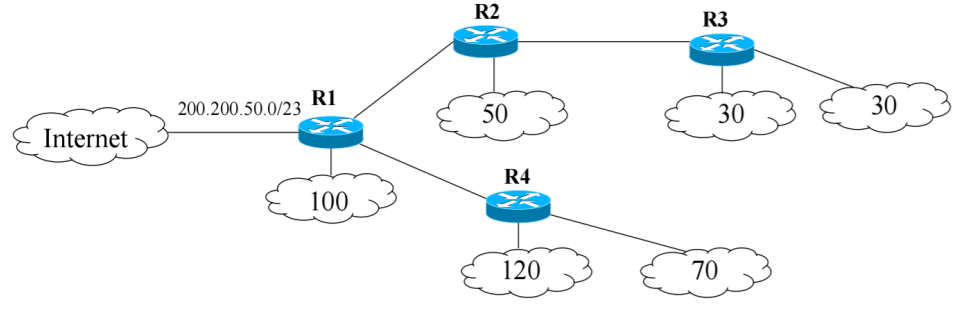
\includegraphics[width=\textwidth]{siec.png}
\caption{Schemat sieci}
\end{figure}

\subsection{Odpowiedź}

200.200.50.0/23 dzielę na podsieci z 128 adresami z maską /25

Dostawca usług R1 wydziela 4 podsieci:
\begin{enumerate}
\item{Podsieć 200.200.50.0/25}
\item{Podsieć 200.200.50.128/25}
\item{Podsieć 200.200.51.0/25}
\item{Podsieć 200.200.51.128/25}
\end{enumerate}


Pierwsza podsieć trafia do dostawcy usług R2.
Druga podsieć zostaje przeznaczona na chmurkę o rozmiarze 100.
Trzecia I czwarta podsieć (łącznie 200.200.51.0/24) trafia do dostawcy R4.

Dostawca usług R2 wydziela 2 podsieci z 64 adresami:
\begin{enumerate}
\item{Podsieć 200.200.50.0/26}
\item{Podsieć 200.200.50.64/26}
\end{enumerate}

Pierwsza podsieć zostaje prezznaczona do dostawcy usług R3.
Druga podsieć zostaje przeznaczona na chmurkę o rozmiarze 50.

Dostawca usług R3 wydziela 2 podsieci z 32 adresami:
\begin{enumerate}
\item{Podsieć 200.200.50.0/27}
\item{Podsieć 200.200.50.32/27}
\end{enumerate}

Obie podsieci zostają przeznaczone na chmurki.

Dostawca usług R4 wydziela 2 podsieci z 128 adresami:
\begin{enumerate}
\item{Podsieć 200.200.51.0/25}
\item{Podsieć 200.200.51.128/25}
\end{enumerate}

Obie podsieci zostają przeznaczone na chmurki.

\section{Zadanie 4}

Dokonaj agregacji poniższych wpisów na routerze R1 tak bardzo jak się da:

\begin{figure}[H]
\centering
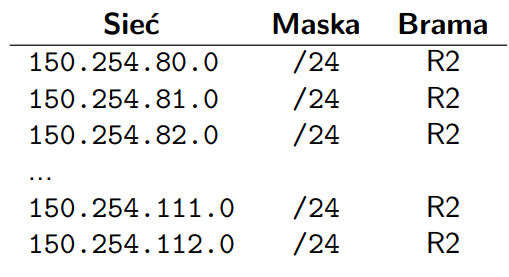
\includegraphics[width=0.5\textwidth]{wpisy router.png}
\caption{Wpisy na routerze R1}
\end{figure}

\subsection{Odpowiedź}

Zagregowane podsieci:
\begin{enumerate}
\item{150.254.80.0/20 / R2}
\item{150.254.96.0/20 / R2}
\item{150.254.112.0/24 / R2}
\end{enumerate}

\end{document}
